\documentclass{f4_beamer}

\title{Convolution und ihre Anwendung in der digitalen Audiobearbeitung}
\subtitle{Seminarfach: Audio DSP}
\author{Julian Mueller \and Tom Nir}
\date{\today}

\usepackage[style=numeric, backend=biber]{biblatex}
\addbibresource{bibliography/bibl.bib}

\begin{document}

% Neue Sektion (Neues Kapitel) in sections.tex einfügen
% Eine Section setzt sich hier aus mehreren Folien (frames) zusammen: \begin{frame}

\section{Grundlagen: Audio DSP}
\label{sec:basics}
\begin{frame}{Sampling}
    \begin{itemize}
        \item Abtastung stetiger Signale $\implies$ Folge diskreter Amplitudenwerte
        \begin{figure}[H]
            \centering
            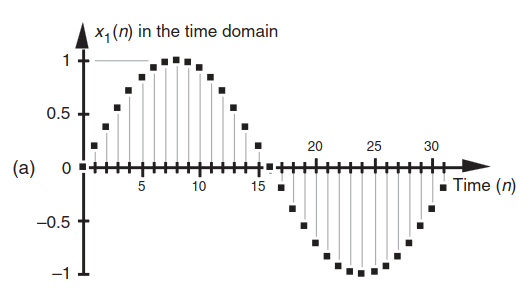
\includegraphics[width=0.6\textwidth]{Graphics/Diskretes_signal_lyons.png}
            \caption{
                Horiz. Achse: Zeitbereich (n-ter Samplewert) 
                Vert. Achse: Amplitude
                }
        \end{figure}
    \end{itemize}
\end{frame}

\section{Literatur}
\begin{frame}[allowframebreaks]{Literaturverzeichnis}
    \printbibliography
\end{frame}


\end{document}
